\documentclass[10pt]{article}
\newcommand{\HRule}{\rule{\linewidth}{0.5mm}}
\parindent 0pt
\parskip 10pt
\usepackage{anysize}
\usepackage{graphicx}
\usepackage{epsfig}
\usepackage{float}
%\usepackage{cite}
\usepackage{natbib}
\usepackage{setspace}
\marginsize{3.5cm}{3.5cm}{1cm}{1cm}
\onehalfspacing
\usepackage{caption}
\usepackage{subcaption}
\usepackage{amsmath,hyperref}

\usepackage{xcolor}
\hypersetup{
    colorlinks,
    linkcolor={red!50!black},
    citecolor={blue!50!black},
    urlcolor={blue!80!black}
}

%\textwidth 15cm
%\textheight 24cm
%\onehalfspacing
\begin{document}

\title{US House Price Analysis: Regression Study}

\author{David Starkey}

\maketitle





\section{House Price Prediction: Introduction and Data Source}



Houses prices are known to vary widely due to an entire range of factors. These are limited not only to the more commonly known attributes such as area, number of bedrooms land acreage etc. More subtle factors also influence the expected property retail price. These might include proximity to a good school, local amenities or whether the area is coastal. This housing data set \footnote{\href{ https://www.kaggle.com/c/house-prices-advanced-regression-techniques/data}{\textcolor{blue}{https://www.kaggle.com/c/house-prices-advanced-regression-techniques/data}}} collects 80 attributes for around 1500 houses sold in the US. The attributes are described alongside the online dataset but include variables such as the age of the property, the land contours or flatness of the property, proximity to a main road and the type of heating system used. This project aims to perform a decision tree random forest regression analysis to predict the expected retail value of a property based on these 80 attributes. The study will also

\begin{itemize}
\item Perform a cross validation to determine the accuracy of the random forest regression.

\item Predict the sale price of a further test sample of 1500 objects with unknown classification.

\item Investigate which of the 80 attributes are the most important in affecting the sale value of the properties in this dataset.

\end{itemize}







\section{Random Forest Regression Analysis}
\label{sec_rf}
This section will detail the statistical algorithm used to classify the data for the interested reader. The layperson is welcome to skip to the results section for the summary of the main finding.

The random forest decision tree classifier is a rather complex algorithm with many steps. A disadvantage to this algorithm (as will become apparent after following the steps below) is that it has a large number of tunable `hyper parameters' that must be set for the decision tree to work. While more simple algorithms like $k$ means clustering are very direct with no `tune-ing' requirements, a random forest requires the user to specify the number of trees in the forest, the depth of each tree, the cost function and in some cases the method by which to assign the class (i.e should we average the probability distributions from each tree or use the mode class from each tree to assign the class). Despite this draw back, however, random forest classifiers are very visual classifiers for a general audience to understand intuitively even if the full details of the algorithm are unclear. They are also quite robust and provide very accurate classifications in general. The algorithm for creating a single tree is as follows:

\begin{itemize}
\item Arrange the dataset into a matrix $X(N,M)$ where each of the $N$ rows corresponds to one example in and $M$ dimensional feature space. You may need to apply `one-hot-encoding' to convert categorical variables into a binary matrix format. Also arrange the prediction values (house prices) into an array $C(M)$.


\item Consider a random set of $K < M$ dimensions in the parameter space and a random subset of $I<N$ points from the data set. 

\item We now need a value $S$ above and below which to split the $I$ considered points. The value of all $I$ points, in each dimension $k \in K$ are considered in turn as the split point $S$.

\item The Cost function for each branch $l$ following the split is given by
\begin{equation}
C_l = \sum_{j=1}^{N_j} \left( y_j - \langle y \rangle \right)^2,
\end{equation}

\noindent where $\langle y \rangle$ denotes the average house price of points in this branch. The total cost function is given by summing $C_l$ over each of the two child branches. The choice of split $S$ is given by considering, in turn, each point in the subset of $I$ rows and $K$ dimensions as the split $S$. The value of the data matrix that minimises $C$ is chosen as the split point $S = X(i,k)$.


\item Repeat this for each child of the above node and continue to deepen the tree up to a desired depth (e.g 5 levels). Each time a new node is considered, chose a new random set of $K$ dimensions and $I$ points to consider for the split quantity. The choice of depth is somewhat arbitrary but the node path terminates once the tree has reached a certain depth or if there are no children in the branch following a split (no more data left to populate the branch).

\end{itemize}

The above algorithm generates a single decision tree. The random forest algorithm works by constructing an arbitrary number of trees (e.g 5, 10, 50) and propagating new test data through each tree. Each tree will yield a new house price and the average is used as the output of the random forest. 





\section{Results and Conclusions}
The random forest decision tree regressor is applied to the house price data using a cross validation approach. Of the original 1500 houses in the data set, 25\% are selected to serve as a mock test-sample to serve as a measure of the accuracy of the simulation. A forest of five trees is constructed according to the algorithm in Section \ref{sec_rf} and the random forest, once trained on the mock training set, is used to predict the house prices of the mock test-data set. An example decision tree is shown in Figure \ref{fig_smalltree} and the result of the fits to the mock test data set is shown in Figure \ref{fig_predict}. Figure \ref{fig_predict} shows that the random forest method accurately estimates the house price for a given test data set across all values. The estimated accuracy, calculated from the mean absolute error, is approximately 89.4\%. 

The random forest regressor can also be used to assess the importance of each of the 80 variables in affecting the house price. The fractional importance for the 10 most important variables is show in Figure \ref{fig_import}. It can be seen that the overall quality of the house accounts has the largest effect on the house price. These 10 attributes and their fractional importances are given in Table \ref{tab_import}. 



Future regression exercises might improve on this data set and attempt to speed up the fits by utilizing only the attributes contributing most of the fractional importance. It does seem that most of the variables in this large dataset have very little affect on house prices and it would be of great interest to extend this to regions in the UK. One would expect the demographics, geography and unique housing design differences between UK and US housing may mean that different features than those presented here become the most important drivers of house price fluctuations. Such studies will be presented in upcoming analyses.


\begin{figure}
\begin{center}
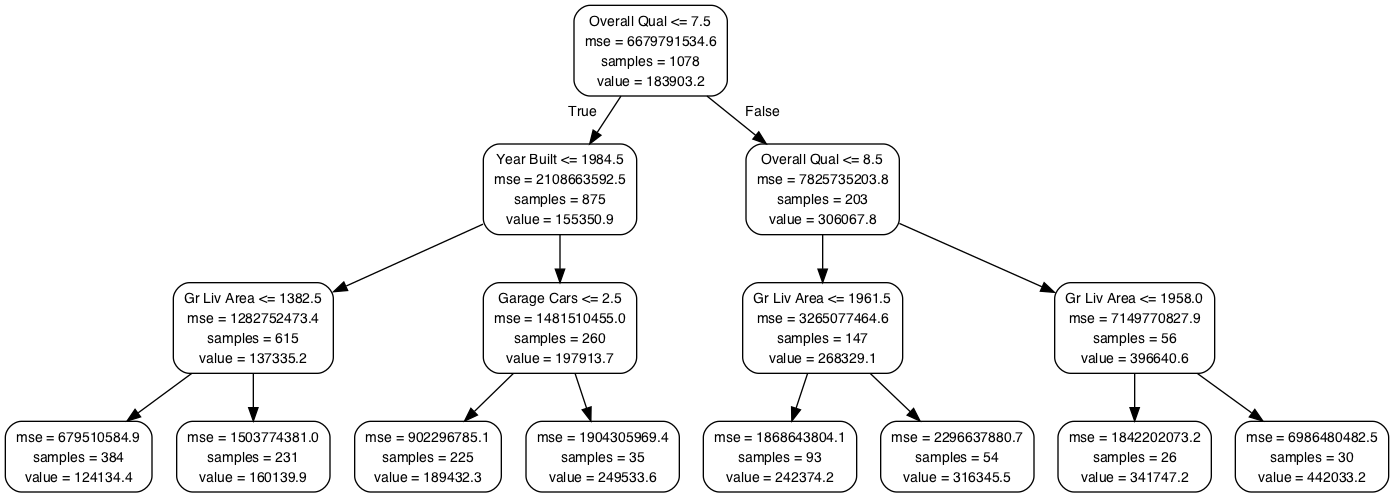
\includegraphics[scale=0.4,angle=0,trim=8cm 0cm 0cm 2cm]{small_tree_0_0.png}
\caption{An example decision tree used to predict the house price. The full tree is much too large to be visualised and so this small example is used as a visual aid.}
\label{fig_smalltree}
\end{center}
\end{figure} 


\begin{figure}
\begin{center}
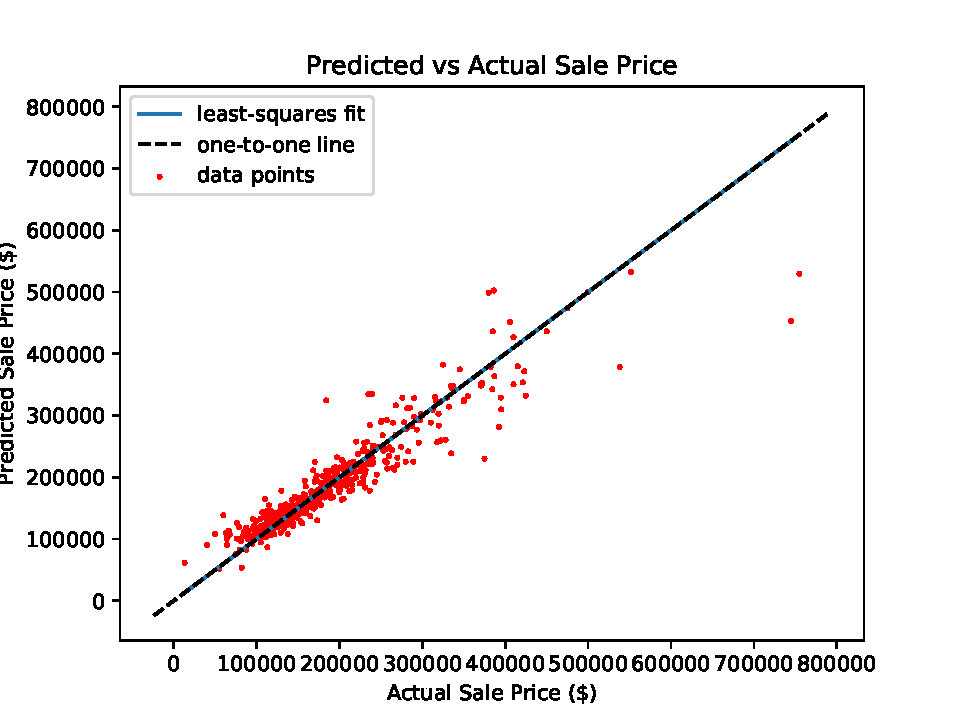
\includegraphics[scale=0.8,angle=0,trim=0cm 0cm 0cm 2cm]{fig_actual_vs_predict.pdf}
\caption{Actual vs Predicted house prices after training of the random forest regression algorithm. The dashed line shows the one-to-one correlation line (a 100\% accurate model with no outlying points would show all point lying on this line).}
\label{fig_predict}
\end{center}
\end{figure} 


\begin{figure}
\begin{center}
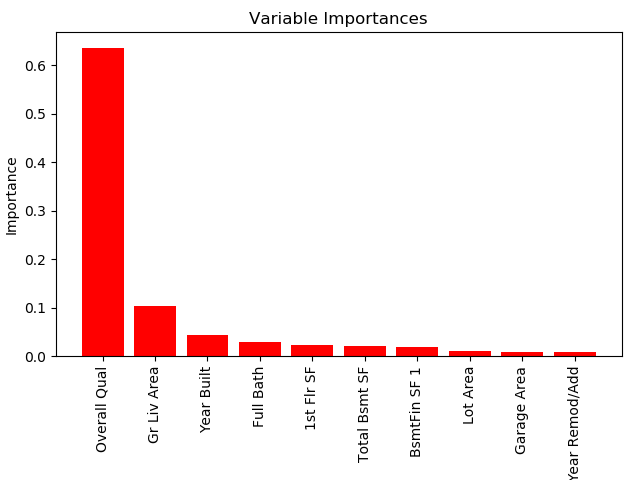
\includegraphics[scale=0.8,angle=0,trim=0cm 0cm 0cm 2cm]{importances_0_0.png}
\caption{Fractional importance of the 10 most important attributes in driving house prices in the US dataset above.}
\label{fig_import}
\end{center}
\end{figure} 






\begin{table}
\center
\caption{Fractional importance of the 10 attributes that most affect the house sale price.}
\begin{tabular}{ccc}
\hline
Attribute & Description & Fractional importance \\
\hline 
\hline
'Overall Qual' & Overall Quality & 0.64 \\
'Gr Liv Area' & Ground Living Area & 0.1 \\
'Year Built' & Year Built & 0.04 \\
'Full Bath' & Number of Bathrooms & 0.03 \\
'1st Flr SF' & 1st Floor Square Footage & 0.02 \\
'Lot Area' & Total Basement Square Footage & 0.02 \\
'Total Bsmt SF' & Basement Finish (Type 1) & 0.02 \\
'Lot Area' & Total lot square footage & 0.01 \\
'Garage Area' & Garage square footage & 0.01 \\
'Year Remod/Add' & Remodelled date & 0.01 \\
\hline
\end{tabular}
\label{tab_import}
\end{table}


\end{document}



